%Compare to phones!
Despite being two very different devices, the mobile phone and Glass, Google's design recommendations are not all that different for the two. Google ask developers who are designing for smartphones to think of simplicity and clarity. Google put much emphasis on making applications easy to use.
\\
\\
There are some differences however. For smartphones Google also recommend that developers keep track of what the users have done in the past. Google ask developers to remember the user's input history and customisation, all to make it easier for the user when they (hopefully) come back to the application.\cite{androidDesignPrinciples}
\\
%\url{https://developer.android.com/design/index.html}\\
%\url{https://developer.android.com/design/get-started/principles.html}
	\begin{figure}[ht!]
		\centering
		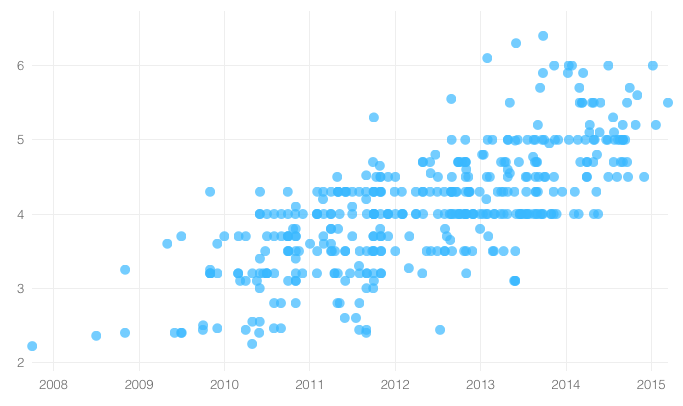
\includegraphics[width=110mm]{images/smartphoneSize}
		\caption{\cite{smartphoneSizeChart}}
		\label{smartphoneSizeChart}
	\end{figure}
	%http://www.pcworld.com/article/2455169/why-smartphone-screens-are-getting-bigger-specs-reveal-a-surprising-story.html
\\
Google differ in how they want developers to design applications for smartphones and Google Glass respectively. Google are much more open to developers using their own ideas when designing for smartphones. Google encourage freedom and give more subtle hints of how to design. For instance Google want developers to make applications fun and easy to use. They recommend consistency and a rewarding application.
\\
\\
Designing for Google Glass comes with a few more restrictions. 

[TODO expand and elaborate with more examples]

% Color schemes
% pre defined layouts
% pre defined typography (fonts)







